% AnimateDiff architecture figure for the Literature Survey.
% Drawn at the report's \textwidth (6.5in = 16.5cm), so it is included at 1:1 and the text sizes are real.
% Build: pdflatex animatediff_arch.tex  ->  animatediff_arch.pdf
\documentclass[tikz,border=1pt]{standalone}
\usepackage{amsmath,amssymb}
\usetikzlibrary{positioning,arrows.meta,fit,backgrounds,calc}

\definecolor{frzF}{HTML}{E9E9E9}\definecolor{frzD}{HTML}{8C8C8C}
\definecolor{trnF}{HTML}{FBD9B5}\definecolor{trnD}{HTML}{C8661B}
\definecolor{perF}{HTML}{CFE0F3}\definecolor{perD}{HTML}{3F6FA8}

\tikzset{
  >={Stealth[length=1.6mm]},
  font=\sffamily\scriptsize,
  S/.style={draw=frzD, fill=frzF, minimum width=0.46cm, minimum height=0.80cm, inner sep=0pt},
  T/.style={draw=frzD, fill=frzF, minimum width=0.20cm, minimum height=0.80cm, inner sep=0pt},
  trn/.style={draw=trnD, fill=trnF},
  per/.style={draw=perD, fill=perF},
  tab/.style={draw=trnD, fill=trnF, minimum height=0.13cm, inner sep=0pt},
  tabfrz/.style={draw=frzD, fill=frzF, dashed, minimum height=0.13cm, inner sep=0pt},
  title/.style={font=\sffamily\footnotesize\bfseries},
  inp/.style={align=center, font=\sffamily\scriptsize, text=black!85},
  note/.style={align=center, text width=3.55cm, font=\sffamily\scriptsize, text=black!80},
  op/.style={draw=trnD, fill=trnF!70, rounded corners=2pt, align=center, minimum height=1.05cm,
             inner sep=2pt, font=\sffamily\scriptsize},
  dimlbl/.style={font=\scriptsize, text=black!75},
  flow/.style={->, draw=black!70, thick},
}

% three stacked frames = a clip, lower-left corner at (#1,#2)
\newcommand{\vclip}[2]{%
  \foreach \i in {2,1,0}{\draw[fill=white, draw=black!55] ($(#1,#2)+(\i*0.06,\i*0.06)$) rectangle ++(0.40,0.27);}}

% three (spatial, temporal) pairs centred on x=#1, bottom at y=#2; #3 #4 = extra styles of S and T; #5 = name prefix
\newcommand{\strip}[5]{%
  \foreach \k in {0,1,2}{%
    \node[S,#3,anchor=south west] (#5S\k) at ($(#1-1.06,#2)+(\k*0.76,0)$) {};
    \node[T,#4,anchor=south west] (#5T\k) at ($(#1-1.06+0.48,#2)+(\k*0.76,0)$) {};}}

\begin{document}
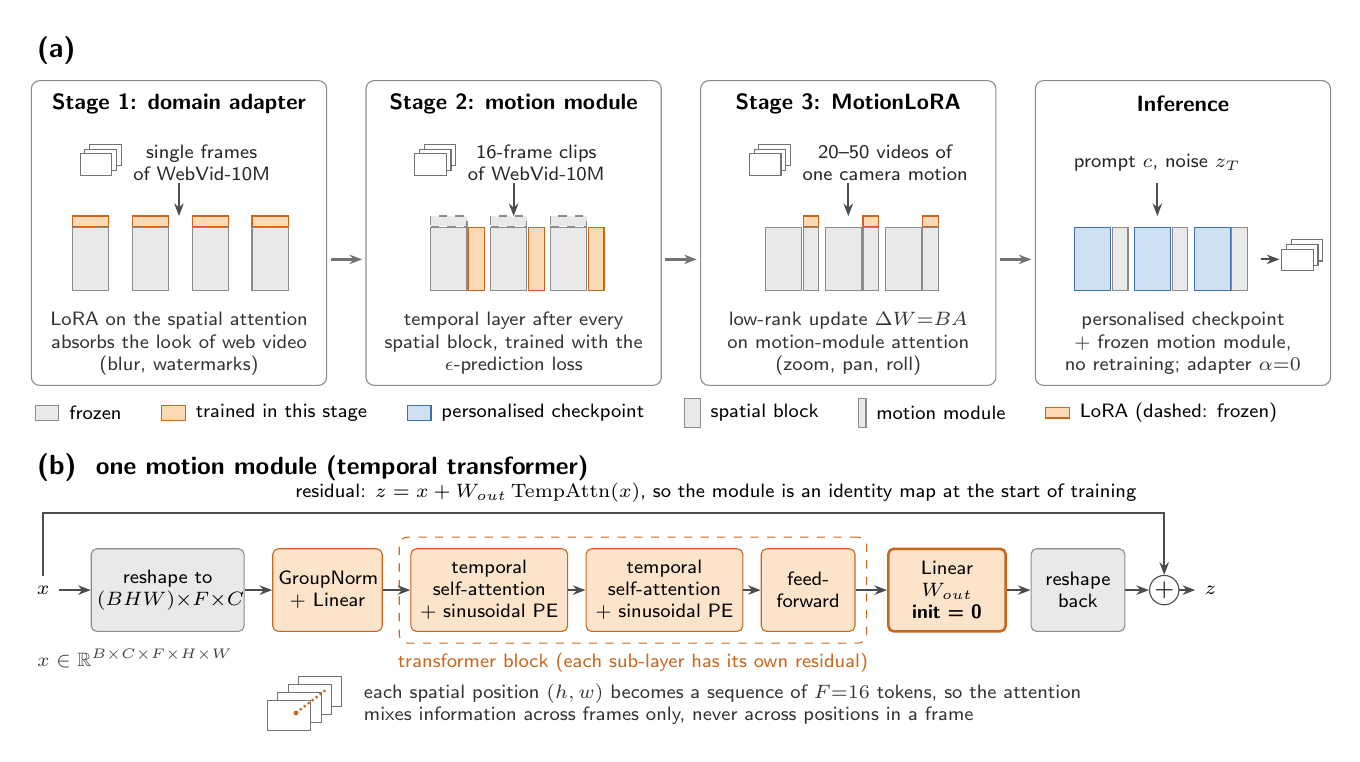
\begin{tikzpicture}

% ---------------- (a) three training stages, then inference ----------------
\def\pw{3.75}\def\gap{0.5}\def\cx{1.875}
\foreach \p in {0,1,2,3}{\coordinate (P\p) at ({\p*(\pw+\gap)},0);}

% Stage 1: domain adapter = LoRA on the frozen image U-Net, trained on single video frames
\begin{scope}[shift={(P0)}]
  \node[title] at (\cx,2.62) {Stage 1: domain adapter};
  \vclip{0.62}{1.72}\node[inp, anchor=west] at (1.17,1.88) {single frames\\of WebVid-10M};
  \draw[flow] (\cx,1.62) -- (\cx,1.20);
  \foreach \k in {0,1,2,3}{%
    \node[S,anchor=south west] (a\k) at ($(\cx-1.36,0.25)+(\k*0.76,0)$) {};
    \node[tab,anchor=south, minimum width=0.46cm] at (a\k.north) {};}
  \node[note, anchor=north] at (\cx,0.10) {LoRA on the spatial attention\\absorbs the look of web video\\(blur, watermarks)};
\end{scope}

% Stage 2: motion modules are the only trained weights
\begin{scope}[shift={(P1)}]
  \node[title] at (\cx,2.62) {Stage 2: motion module};
  \vclip{0.62}{1.72}\node[inp, anchor=west] at (1.17,1.88) {16-frame clips\\of WebVid-10M};
  \draw[flow] (\cx,1.62) -- (\cx,1.20);
  \strip{\cx}{0.25}{}{trn}{b}
  \foreach \k in {0,1,2}{\node[tabfrz,anchor=south, minimum width=0.46cm] at (bS\k.north) {};}
  \node[note, anchor=north] at (\cx,0.10) {temporal layer after every\\spatial block, trained with the\\$\epsilon$-prediction loss};
\end{scope}

% Stage 3: MotionLoRA on the frozen motion modules
\begin{scope}[shift={(P2)}]
  \node[title] at (\cx,2.62) {Stage 3: MotionLoRA};
  \vclip{0.62}{1.72}\node[inp, anchor=west] at (1.17,1.88) {20--50 videos of\\one camera motion};
  \draw[flow] (\cx,1.62) -- (\cx,1.20);
  \strip{\cx}{0.25}{}{}{c}
  \foreach \k in {0,1,2}{\node[tab,anchor=south, minimum width=0.20cm] at (cT\k.north) {};}
  \node[note, anchor=north] at (\cx,0.10) {low-rank update $\Delta W{=}BA$\\on motion-module attention\\(zoom, pan, roll)};
\end{scope}

% Inference: motion module plugged into a personalised checkpoint, no retraining
\begin{scope}[shift={(P3)}]
  \node[title] at (\cx,2.62) {Inference};
  \node[inp] at (1.55,1.88) {prompt $c$, noise $z_T$};
  \draw[flow] (1.55,1.62) -- (1.55,1.20);
  \strip{1.55}{0.25}{per}{}{d}
  \draw[flow] (2.86,0.65) -- (3.10,0.65);
  \vclip{3.13}{0.51}
  \node[note, anchor=north] at (\cx,0.10) {personalised checkpoint\\+ frozen motion module,\\no retraining; adapter $\alpha{=}0$};
\end{scope}

% panel frames and arrows between panels
\foreach \p in {0,1,2,3}{\draw[black!45, rounded corners=3pt] ($(P\p)+(0,-0.95)$) rectangle ($(P\p)+(\pw,2.92)$);}
\foreach \p/\q in {0/1,1/2,2/3}{\draw[->, very thick, black!55] ($(P\p)+(\pw+0.05,0.65)$) -- ($(P\q)+(-0.05,0.65)$);}

% legend, laid out left to right
\node[S, minimum width=0.30cm, minimum height=0.20cm] (l1) at (0.20,-1.30) {};
\node[anchor=west] (L1) at (l1.east) {frozen};
\node[S, trn, minimum width=0.30cm, minimum height=0.20cm, right=0.38cm of L1] (l2) {};
\node[anchor=west] (L2) at (l2.east) {trained in this stage};
\node[S, per, minimum width=0.30cm, minimum height=0.20cm, right=0.38cm of L2] (l3) {};
\node[anchor=west] (L3) at (l3.east) {personalised checkpoint};
\node[S, minimum width=0.20cm, minimum height=0.36cm, right=0.38cm of L3] (l4) {};
\node[anchor=west] (L4) at (l4.east) {spatial block};
\node[T, minimum width=0.09cm, minimum height=0.36cm, right=0.38cm of L4] (l5) {};
\node[anchor=west] (L5) at (l5.east) {motion module};
\node[tab, minimum width=0.30cm, right=0.38cm of L5] (l6) {};
\node[anchor=west] (L6) at (l6.east) {LoRA (dashed: frozen)};

\node[font=\sffamily\normalsize\bfseries, anchor=south west] at (-0.05,3.0) {(a)};

% ---------------- (b) inside one motion module ----------------
\begin{scope}[shift={(0,-3.55)}]
  \node[font=\sffamily\normalsize\bfseries, anchor=west] (blab) at (-0.05,1.55) {(b)};
  \node[font=\sffamily\small\bfseries, anchor=west] at (blab.east) {one motion module (temporal transformer)};

  \node (x) at (0.15,0) {$x$};
  \node[dimlbl, anchor=north west] at (-0.05,-0.62) {$x \in \mathbb{R}^{B\times C\times F\times H\times W}$};
  \node[op, draw=frzD, fill=frzF, right=0.40cm of x, text width=1.8cm] (r1) {reshape to\\$(BHW){\times}F{\times}C$};
  \node[op, right=0.35cm of r1, text width=1.25cm] (gn) {GroupNorm\\+ Linear};
  \node[op, right=0.35cm of gn, text width=1.85cm] (a1) {temporal\\self-attention\\+ sinusoidal PE};
  \node[op, right=0.22cm of a1, text width=1.85cm] (a2) {temporal\\self-attention\\+ sinusoidal PE};
  \node[op, right=0.22cm of a2, text width=1.05cm] (ff) {feed-\\forward};
  \node[op, right=0.40cm of ff, text width=1.35cm, line width=0.9pt] (wo) {Linear $W_{out}$\\\textbf{init = 0}};
  \node[op, draw=frzD, fill=frzF, right=0.30cm of wo, text width=1.05cm] (r2) {reshape\\back};
  \node[draw=black!70, circle, inner sep=0.4pt, right=0.30cm of r2, font=\small] (plus) {$+$};
  \node[right=0.20cm of plus] (z) {$z$};

  \begin{scope}[on background layer]
    \node[draw=trnD, dashed, rounded corners=3pt, fit=(a1)(a2)(ff), inner sep=4pt,
          label={[font=\sffamily\scriptsize, text=trnD]below:transformer block (each sub-layer has its own residual)}] (tb) {};
  \end{scope}

  \draw[flow] (x) -- (r1); \draw[flow] (r1) -- (gn);
  \draw[flow] (gn) -- (a1); \draw[flow] (a1) -- (a2); \draw[flow] (a2) -- (ff); \draw[flow] (ff) -- (wo);
  \draw[flow] (wo) -- (r2); \draw[flow] (r2) -- (plus); \draw[flow] (plus) -- (z);
  \draw[flow] (x.north) -- ++(0,0.80) -| (plus.north)
     node[pos=0.3, above=0pt, font=\sffamily\scriptsize]
     {residual: $z = x + W_{out}\,\mathrm{TempAttn}(x)$, so the module is an identity map at the start of training};

  % what the reshape does: one spatial position across the F frames becomes a token sequence
  \begin{scope}[shift={(3.0,-1.78)}]
    \foreach \i in {3,2,1,0}{%
      \draw[fill=white, draw=black!55] (\i*0.13,\i*0.10) rectangle ++(0.55,0.38);
      \fill[trnD] ($(\i*0.13,\i*0.10)+(0.36,0.22)$) circle (0.03);}
    \draw[trnD, densely dotted, thick] (0.36,0.22) -- ($(3*0.13,3*0.10)+(0.36,0.22)$);
    \node[anchor=west, align=left, text=black!80] at (1.10,0.33)
      {each spatial position $(h,w)$ becomes a sequence of $F{=}16$ tokens, so the attention\\mixes information across frames only, never across positions in a frame};
  \end{scope}
\end{scope}

\end{tikzpicture}
\end{document}
